\subsection{Related Work}
\label{sec:naysayer-related}

 \begin{figure}[tbh]
    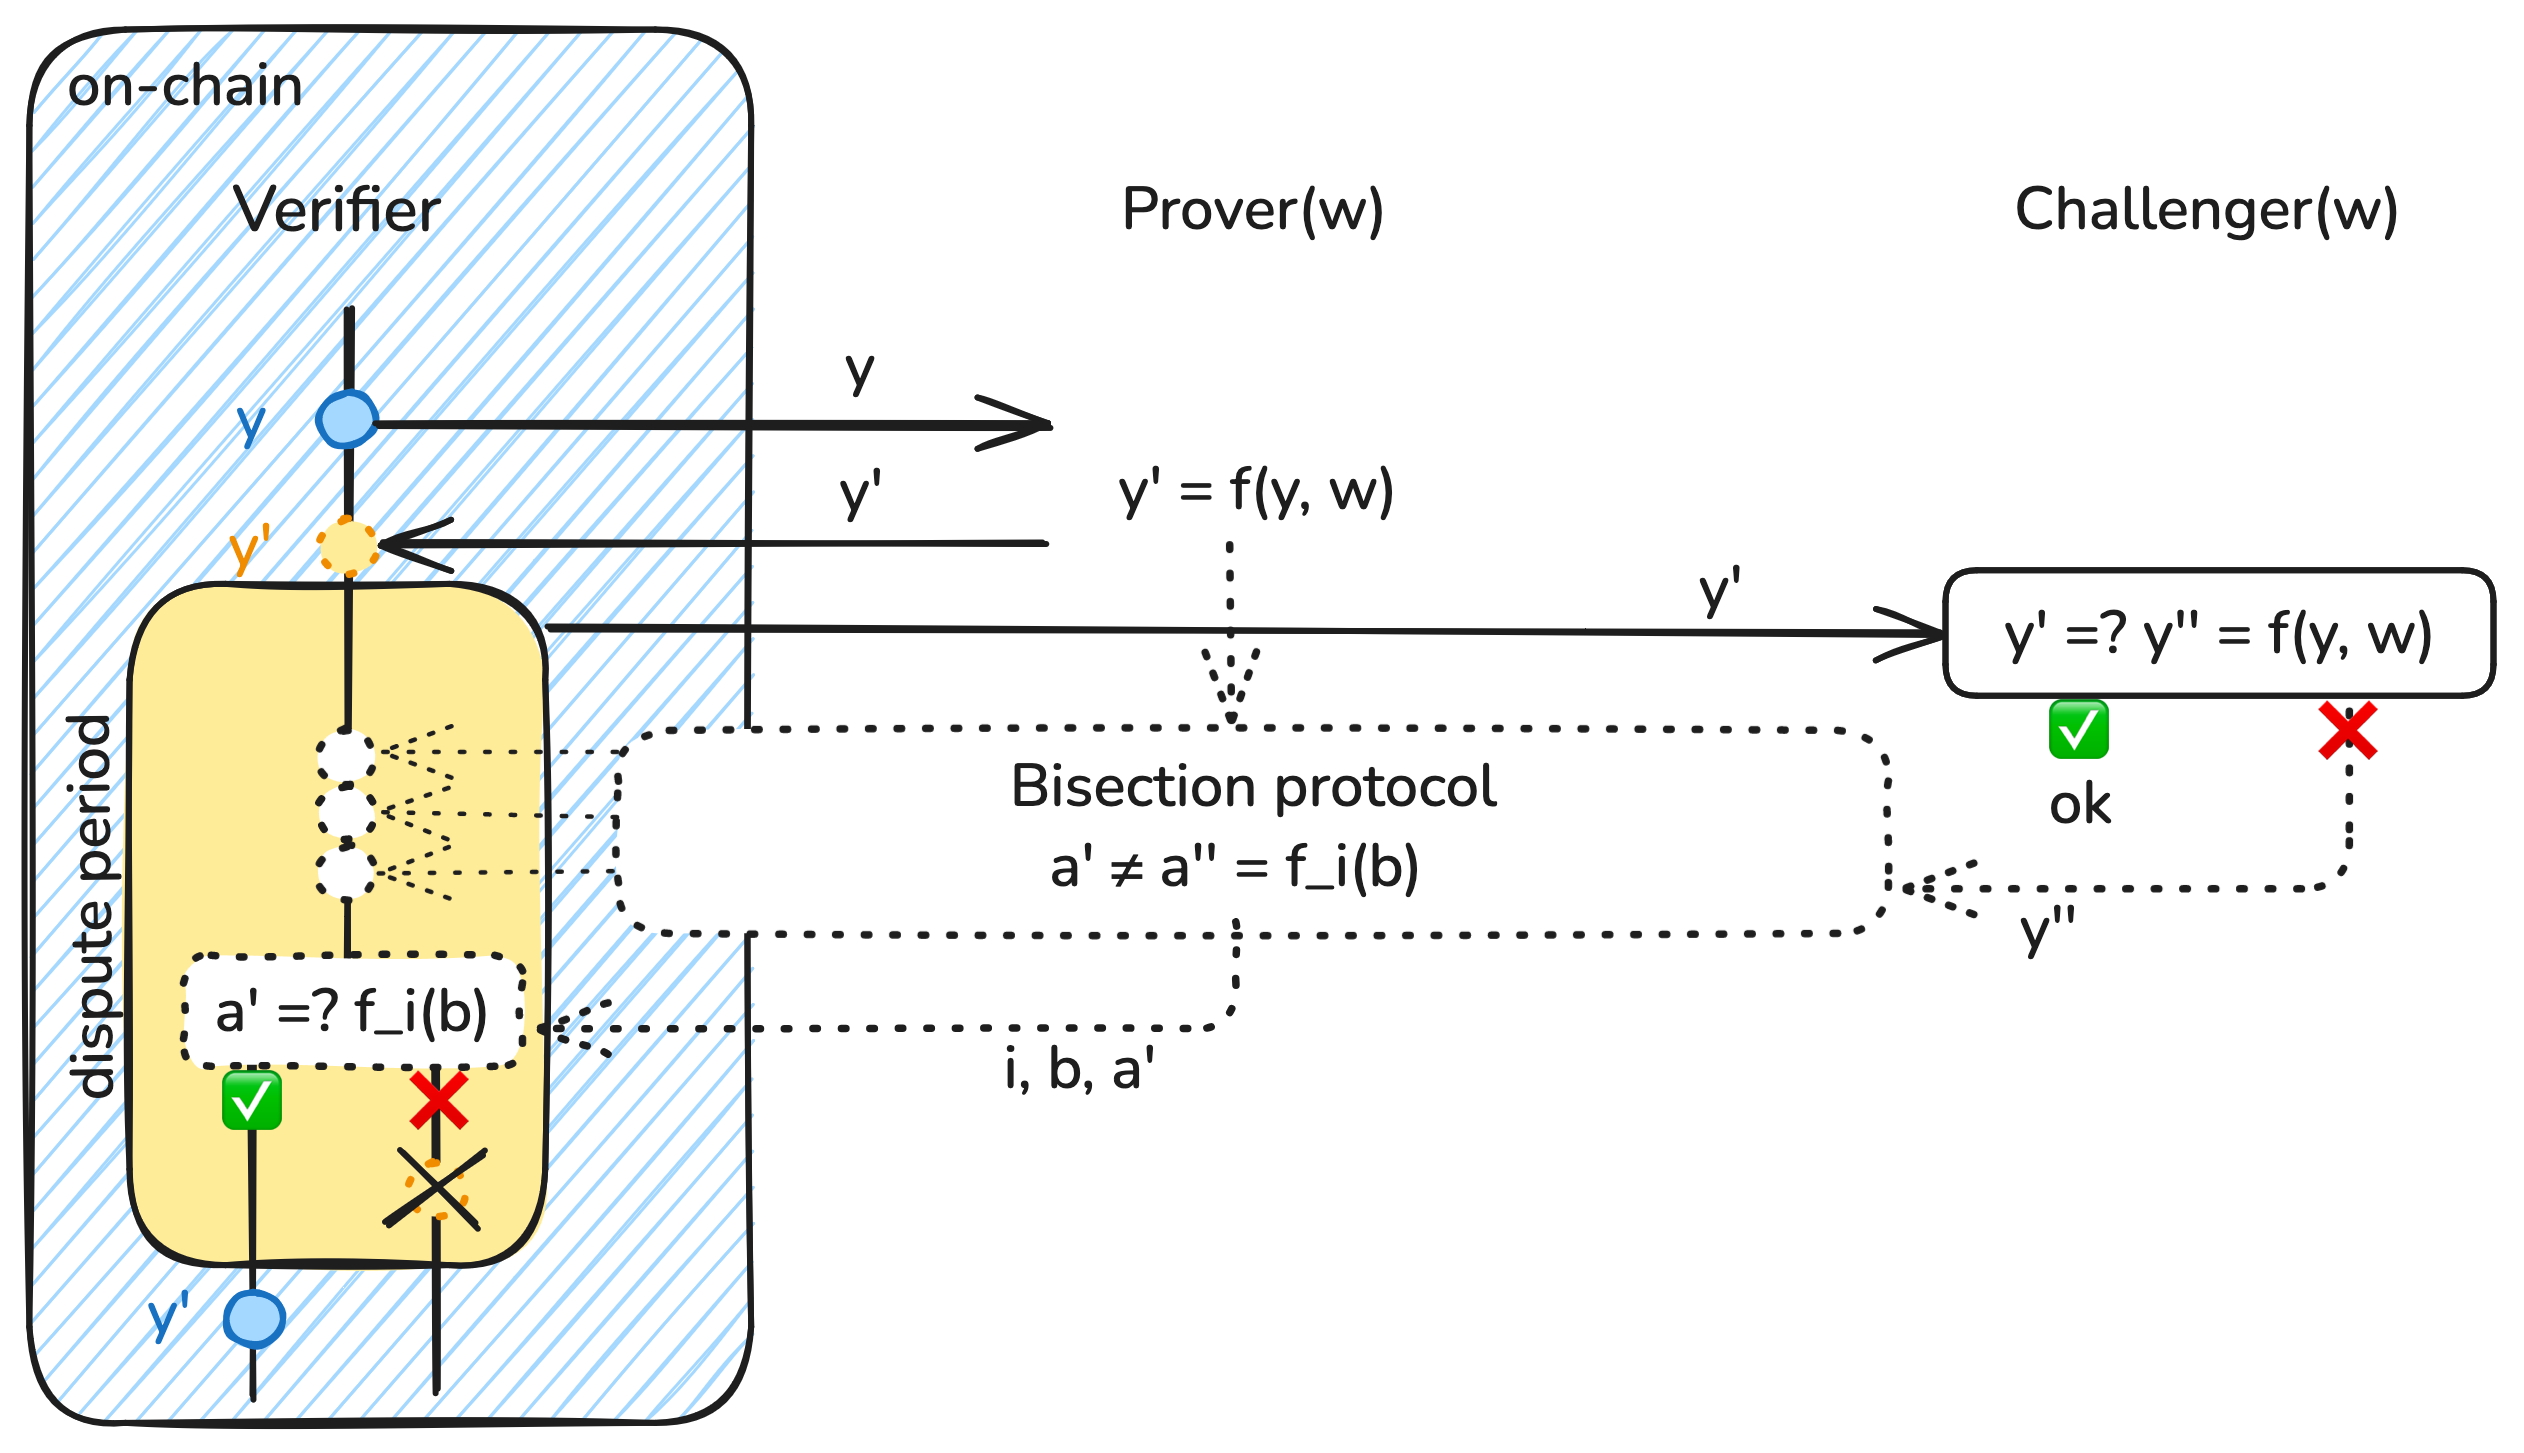
\includegraphics[width=\textwidth]{naysayer/figs/fraud-interactive.png}
    \caption{\textbf{Interactive fraud ``proofs''.} Like naysayer proofs, fraud ``proofs'' make use of challengers and challenge periods. Again, the off-chain ``prover'' computes $y' = f(y, w)$, but without providing any proof of correctness $\pi$. During the challenge period, anyone (with access to $w$, e.g., the batch of transactions) can re-compute $f(y, w)$. If the result $y''$ does not equal $y'$, the party engages in a bisection protocol with the original ``prover'' to narrow the disagreement to a single step of the computation $f_i(b)$. The defender and challenger submit their respective one-step results $a' \neq a''$ to the on-chain verifier, who re-executes $f_i(b)$ on-chain. Based on the result, it may reject the original claim $y'$. If the challenge period elapses without any successful fraud proofs, $y'$ is accepted.}
    \label{fig:fraud-interactive}
 \end{figure}

 \begin{figure}[tbh]
    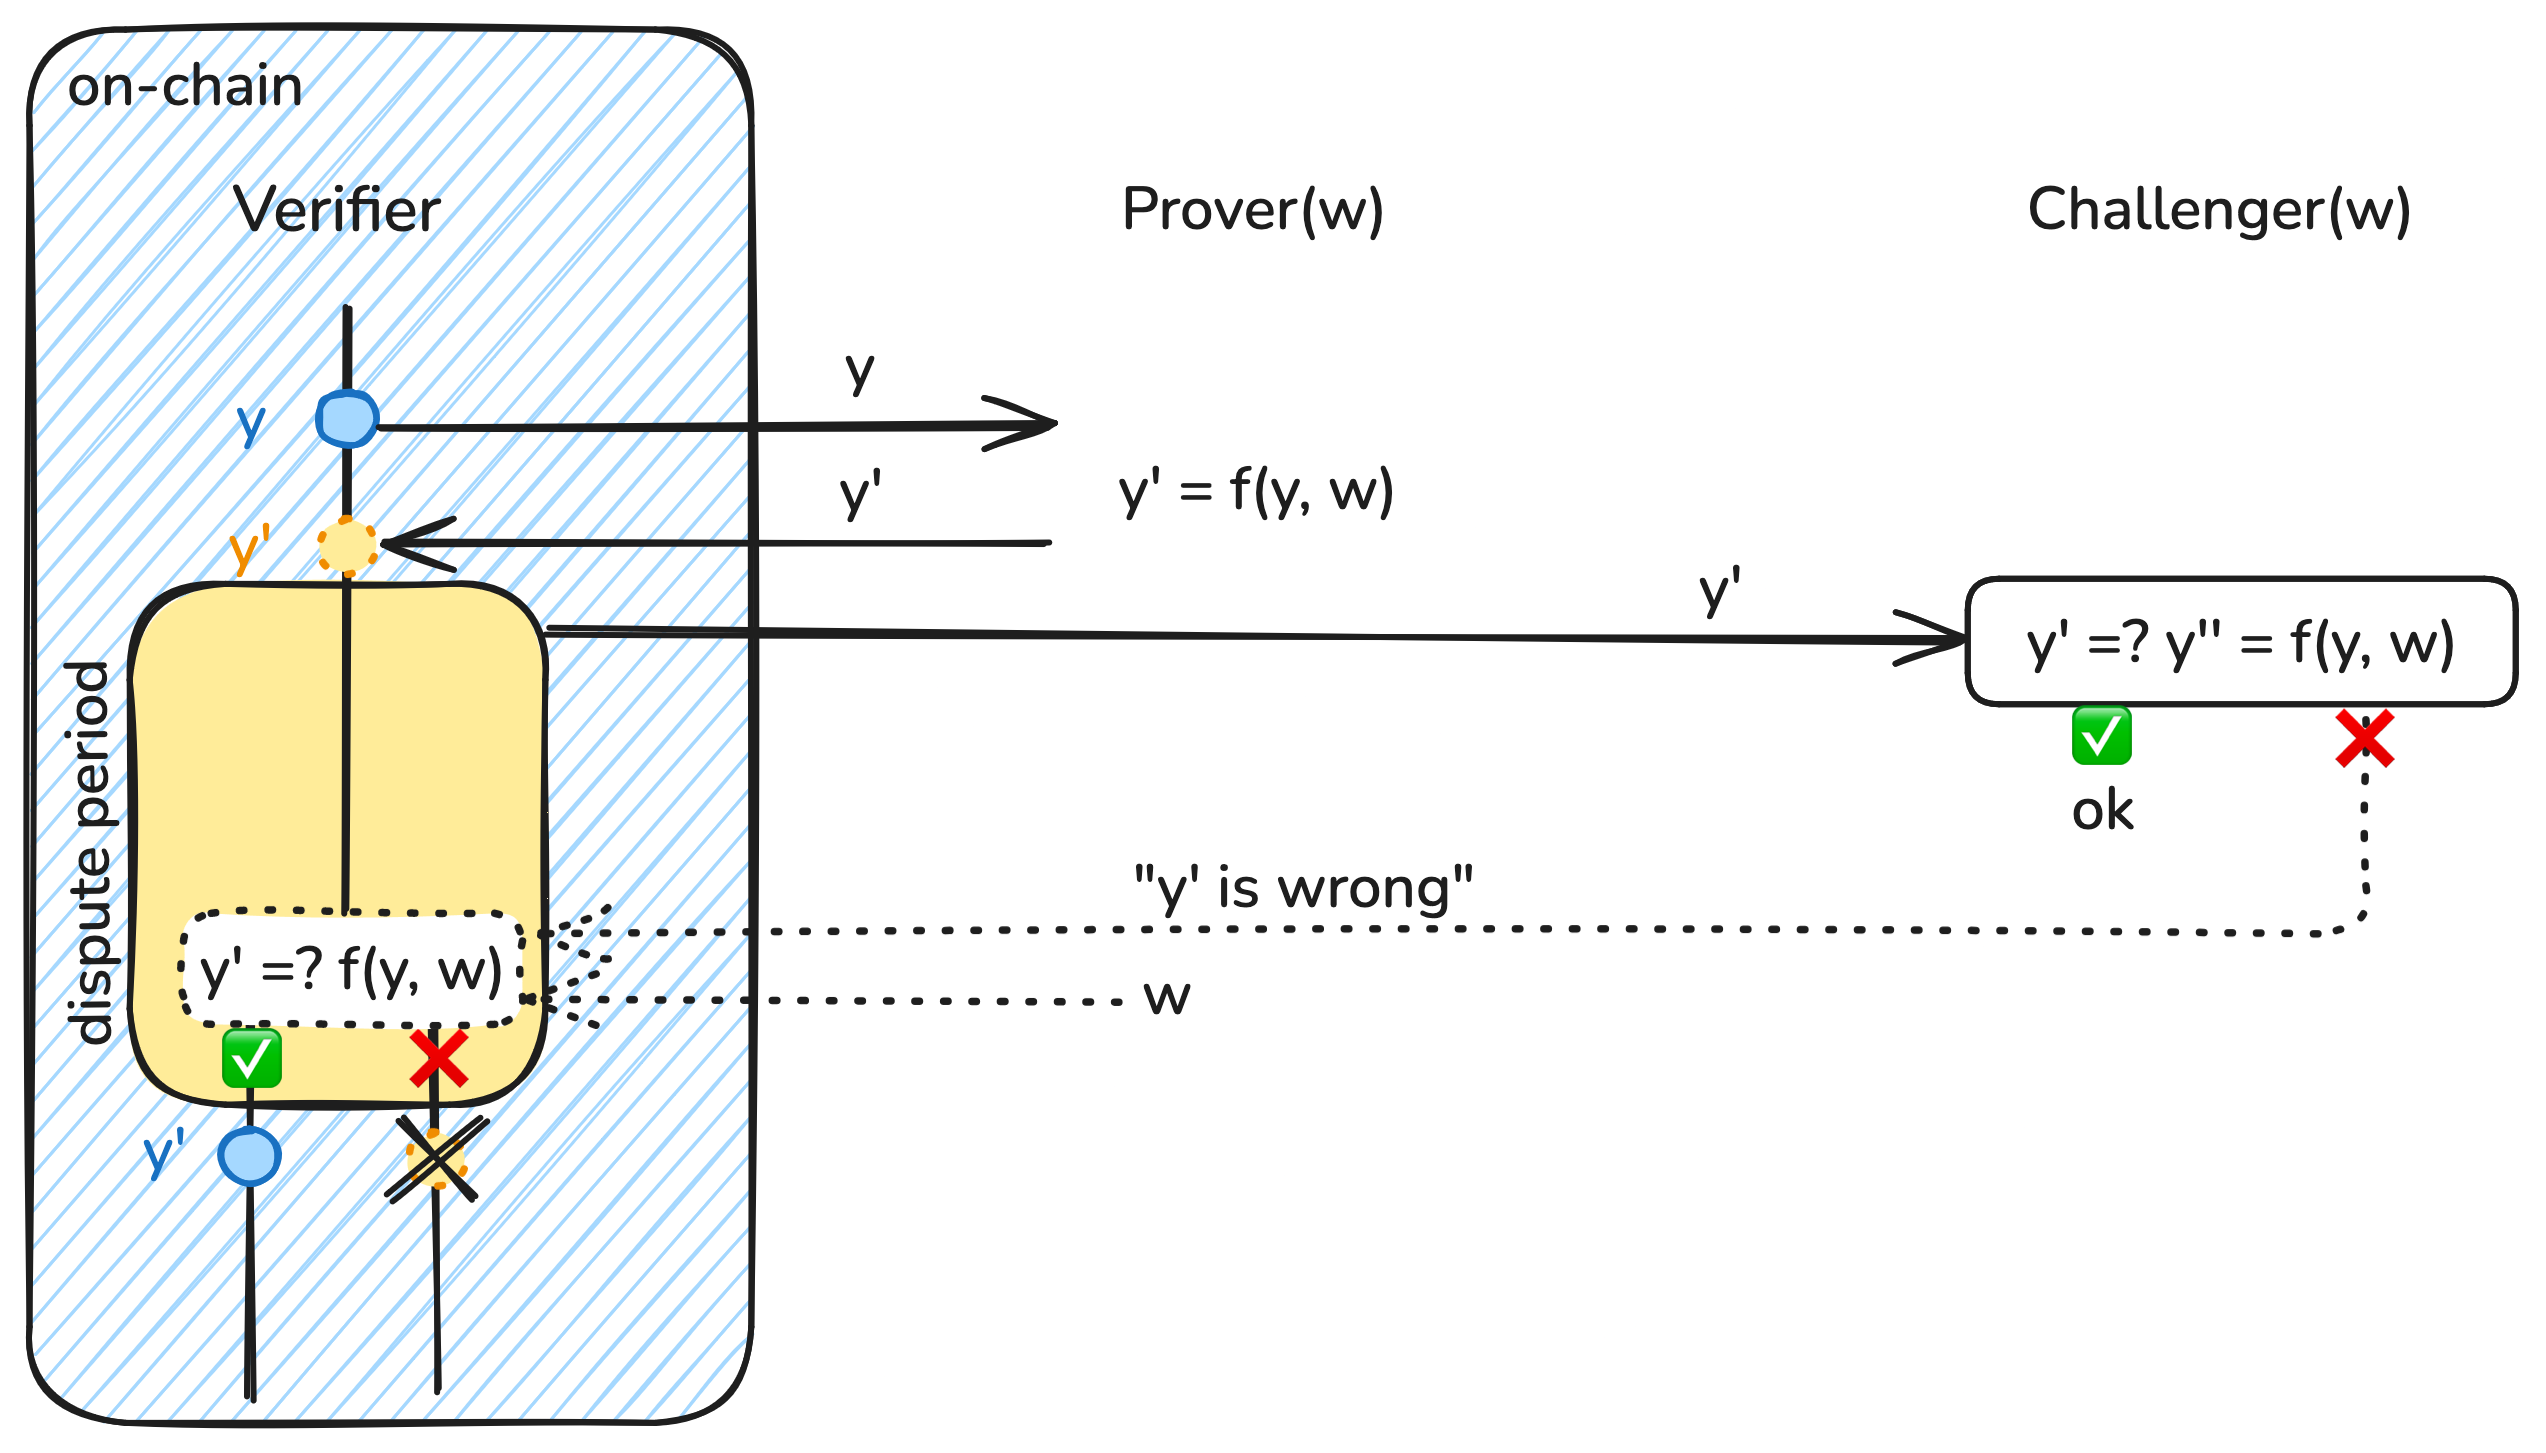
\includegraphics[width=\textwidth]{naysayer/figs/fraud-NI.png}
    \caption{\textbf{Non-interactive fraud ``proofs''.} The non-interactive version functions similarly, except that there is no bisection game. Instead, the on-chain verifier simply re-executes the entire computation $f(y, w)$ on-chain to decide whether or not to reject $y'$. Again, if the challenge period elapses without any challenges, $y'$ is accepted.}
    \label{fig:fraud-NI}
 \end{figure}

A concept related to the naysayer paradigm is \emph{refereed delegation}~\cite{STOC:FeiKil97}. The idea has found widespread adoption~\cite{ARXIV:TeuRei19,USENIX:KGCWF18} under the name ``fraud proofs'' or ``fault proofs'' and is the core idea behind \emph{optimistic rollups}~\cite{ethereum_optimistic,arbitrum_nitro,optimism_rollup}. In classic refereed delegation, a server can output a heavy computation to two external parties, who independently compute and return the result. If the reported results disagree, the parties engage in a \emph{bisection protocol} which pinpoints the single step of the computation which gave rise to the disagreement by recursively halving the computational trace (essentially performing a binary search). Once the discrepancy has been reduced to a single step of the computation, the original server can re-execute only that step to determine which of the two parties' results is correct. 

In the context of optimistic rollups, a ``prover'' performs the computation off-chain and posts the result on-chain, where it is provisionally accepted. Any party can then challenge the correctness of the result by posting a challenge on-chain and engaging in the bisection protocol with the prover via on-chain messages (\Cref{fig:fraud-interactive}). (The term ``fraud proof'' or ``fault proof'' refers to these messages.\footnote{Note that, despite the name, this is not actually a proof system, nor does it depend on any proof system.}) Once the problematic step is identified, it is re-executed on-chain to resolve the dispute. A dispute can also be resolved \emph{non-interactively} by re-running the entire computation on-chain in the event of a dispute (\Cref{fig:fraud-NI}), an approach initially taken by Optimism~\cite{optimism_v1,fraudproofs_medium}.

If no one challenges the prover's result before the end of the \emph{challenge period} (typically 7 days), it is accepted and irreversibly commited on the layer-1 chain.

%Commented out for flow and space
%To improve usability and modularity, researchers have even suggested using succinct proofs of the disputed computation or computation step, replacing the potentially costly on-chain re-execution with proof verification~\cite{buckland_fraudproofs}.

% https://medium.com/@cpbuckland88/fraud-proofs-and-virtual-machines-2826a3412099
% https://www.alchemy.com/overviews/optimistic-rollups

\begin{table}[t]
    \setlength\tabcolsep{0.5em}
    \centering
    \makebox[\linewidth]{
    \begin{tabular}{lcccc}
    \toprule
                                   & VC       & fraud proof       & fraud proof       & naysayer proof \\
                                   &           &   (interactive)   & (non-interactive) &                \\\midrule
        No optimistic assumption   & \yes      & \no               & \no               & \no            \\
        Non-interactive            & \yes      & \no               & \yes              & \yes           \\
        Off-chain $f$  & \yes       & \yes              & \halfcirc             & \yes           \\
        Off-chain $\Pi.\vrfy$  & \no       & -             & -            & \yes           \\
        Witness-independent challenge& \yes    & \no              & \no               & \yes           \\
        Witness-independent resolution& \yes    & \halfcirc              & \no               & \yes           \\
        No $\Pi.\prove$     & \no       & \yes             & \yes              & \no\\
        \bottomrule
    \end{tabular}}
    \caption{Trade-offs between VC, fraud proofs, and naysayer proofs.}
    \label{tab:comparison}
\end{table}

\todo{pick up here}

We compare classic verifiable computation, fraud proofs, and our new approach in \Cref{tab:comparison}. 
Both fraud proofs and naysayer proofs work under an optimistic assumption, i.e., a computation is assumed to be correct unless some party challenges it. 
\noemi{Discuss table here. Note that VC and naysayers require running (cost-intensive) underlying prover, something which fraud proofs avoid.}
At a high level, in the fraud proof paradigm, a ``prover'' performs a provisionally accepted computation without any proof of correctness. Any party can then challenge the correctness of the prover's \emph{computation}. %, potentially by specifying the disputed step of the computation.
In the naysayer paradigm, by contrast, the prover supplies a proof with the computation output, which is provisionally accepted. Any party can then challenge the correctness of the \emph{proof}. %, potentially by specifying the disputed step of the \emph{verification} computation. 
The naysayer approach offers significant speedups since the verifier's circuit is typically much smaller than the original computation. 
Note that there is a slight semantic difference: fraud proofs can definitively show that the computation output is incorrect. In contrast, naysayer proofs can only show that the accompanying proof is invalid---the computation itself may have been correct.

Furthermore, for fraud proofs, the full computation input (the witness) must be made available to the verifier and potential challengers. %and the verifier must be made available to the verifier to settle the dispute. 
Naysayer proofs, on the other hand, 
% are completely stateless to verify:
can be verified using only the statement and proof. 
%\noemi{We have referred to this as ``stateless'', but it's more like no \emph{private} state (i.e. witness) --- is this a standard interpretation of ``stateless'' or might using that word lead to confusion?}
%the on-chain verifier only needs the statement and the proof to check that the proof verifies, and both of these are already available on-chain.
Hence, naysayer proofs work naturally with zero-knowledge proofs.
This can also lead to crucial savings if the witness is very large %as in many cases, the witness is extremely large and, therefore, costly to store on-chain 
(e.g., transaction data for a rollup).

The fraud proof design pattern has been applied in an application-specific way in many blockchain applications besides optimistic rollups, including the Lightning Network~\cite{PooDry16}, Plasma~\cite{PooBut17}, cryptocurrency mixers~\cite{EPRINT:SNBB19}, and distributed key generation~\cite{EPRINT:SJSW19}. We view naysayer proofs as a drop-in replacement for the many application-specific fault proofs, offering an alternative which is both more general and more efficient.

